\chapter{Object Detection}

\paragraph*{}
Following our project plan and discussions with our advisor, the initial phase of our object detection simulation involves identifying a symmetrical target that does not require pose estimation. We selected a cube with a distinct color for ease of detection, specifically a yellow box in the Webots simulation environment.

\paragraph*{}
We conducted \textbf{two different Webots simulations} for this phase. The first simulation uses the built-in recognition node available in the Webots camera device to detect the object. This helps us understand how each robot identifies the object and how it responds post-detection, while also addressing potential challenges such as object occlusion and varying object orientations. 

\paragraph*{}
The second simulation focuses exclusively on object detection using a basic model, specifically HSV color detection in OpenCV, to compare results with the first approach.

\section {The First Simulation}
\textit {Understanding the big picture and challenges}

\begin{figure}[H]
    \centering
    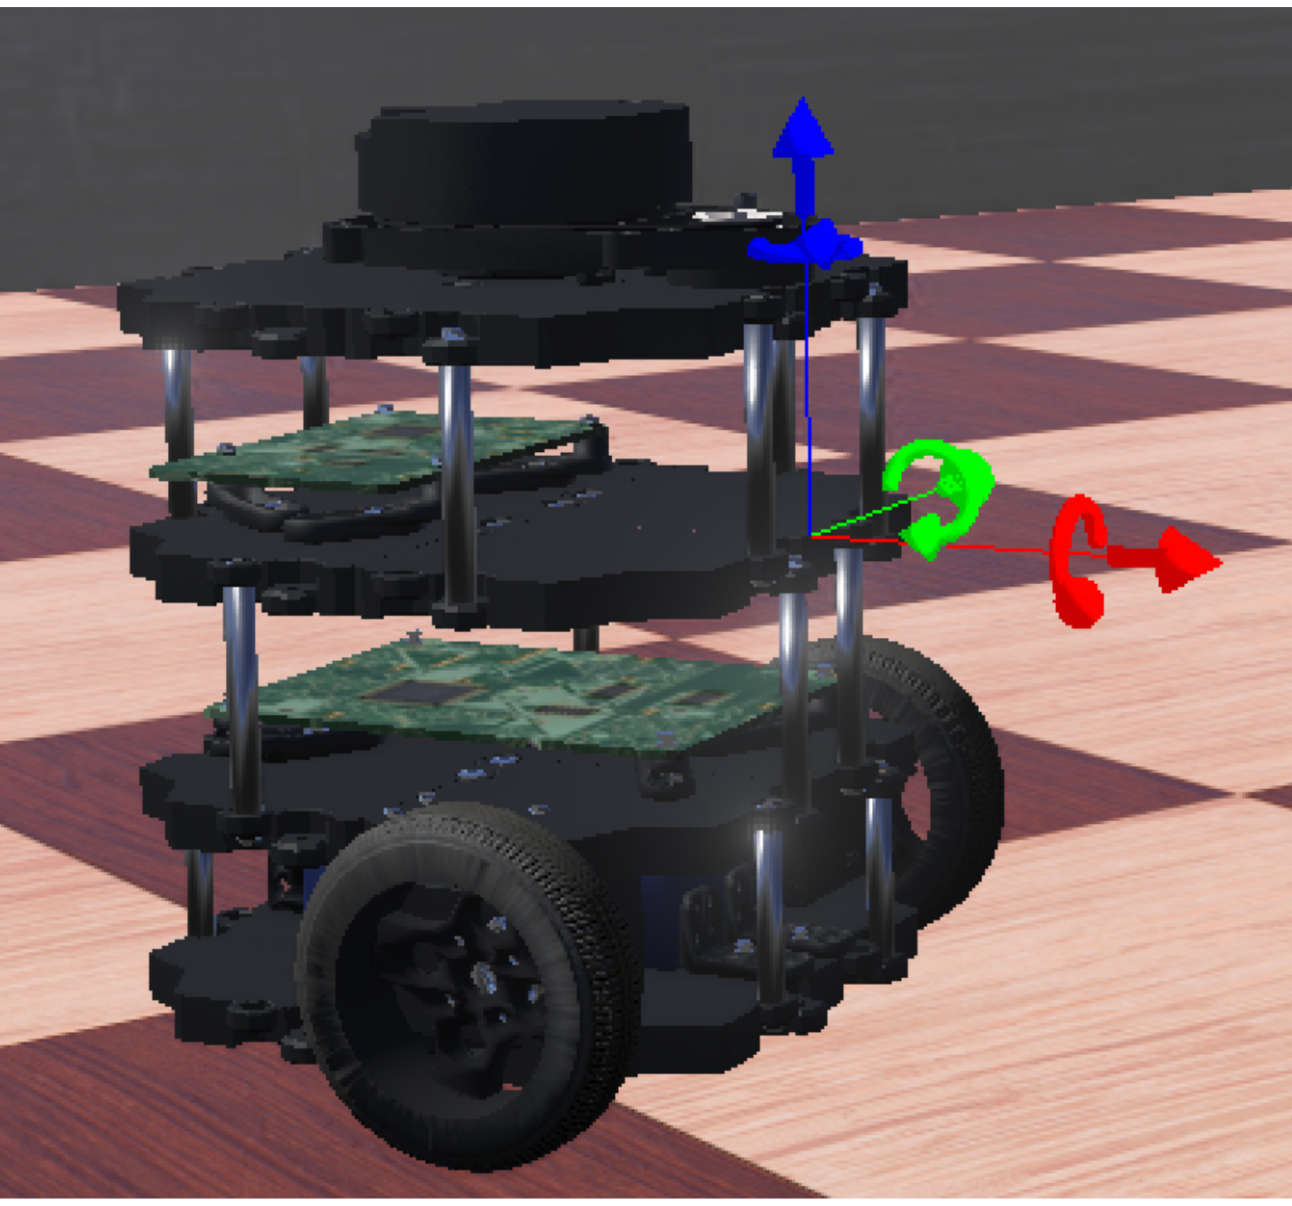
\includegraphics[width=0.6\linewidth]{assets/images/object_detection/Figure1.png}
    \caption{The RGB camera and the rangefinder in the form of a point attached on the TurtleBots}
    \label{fig:object detection figure 1.} 
\end{figure}

\begin{figure}[H]
    \centering
    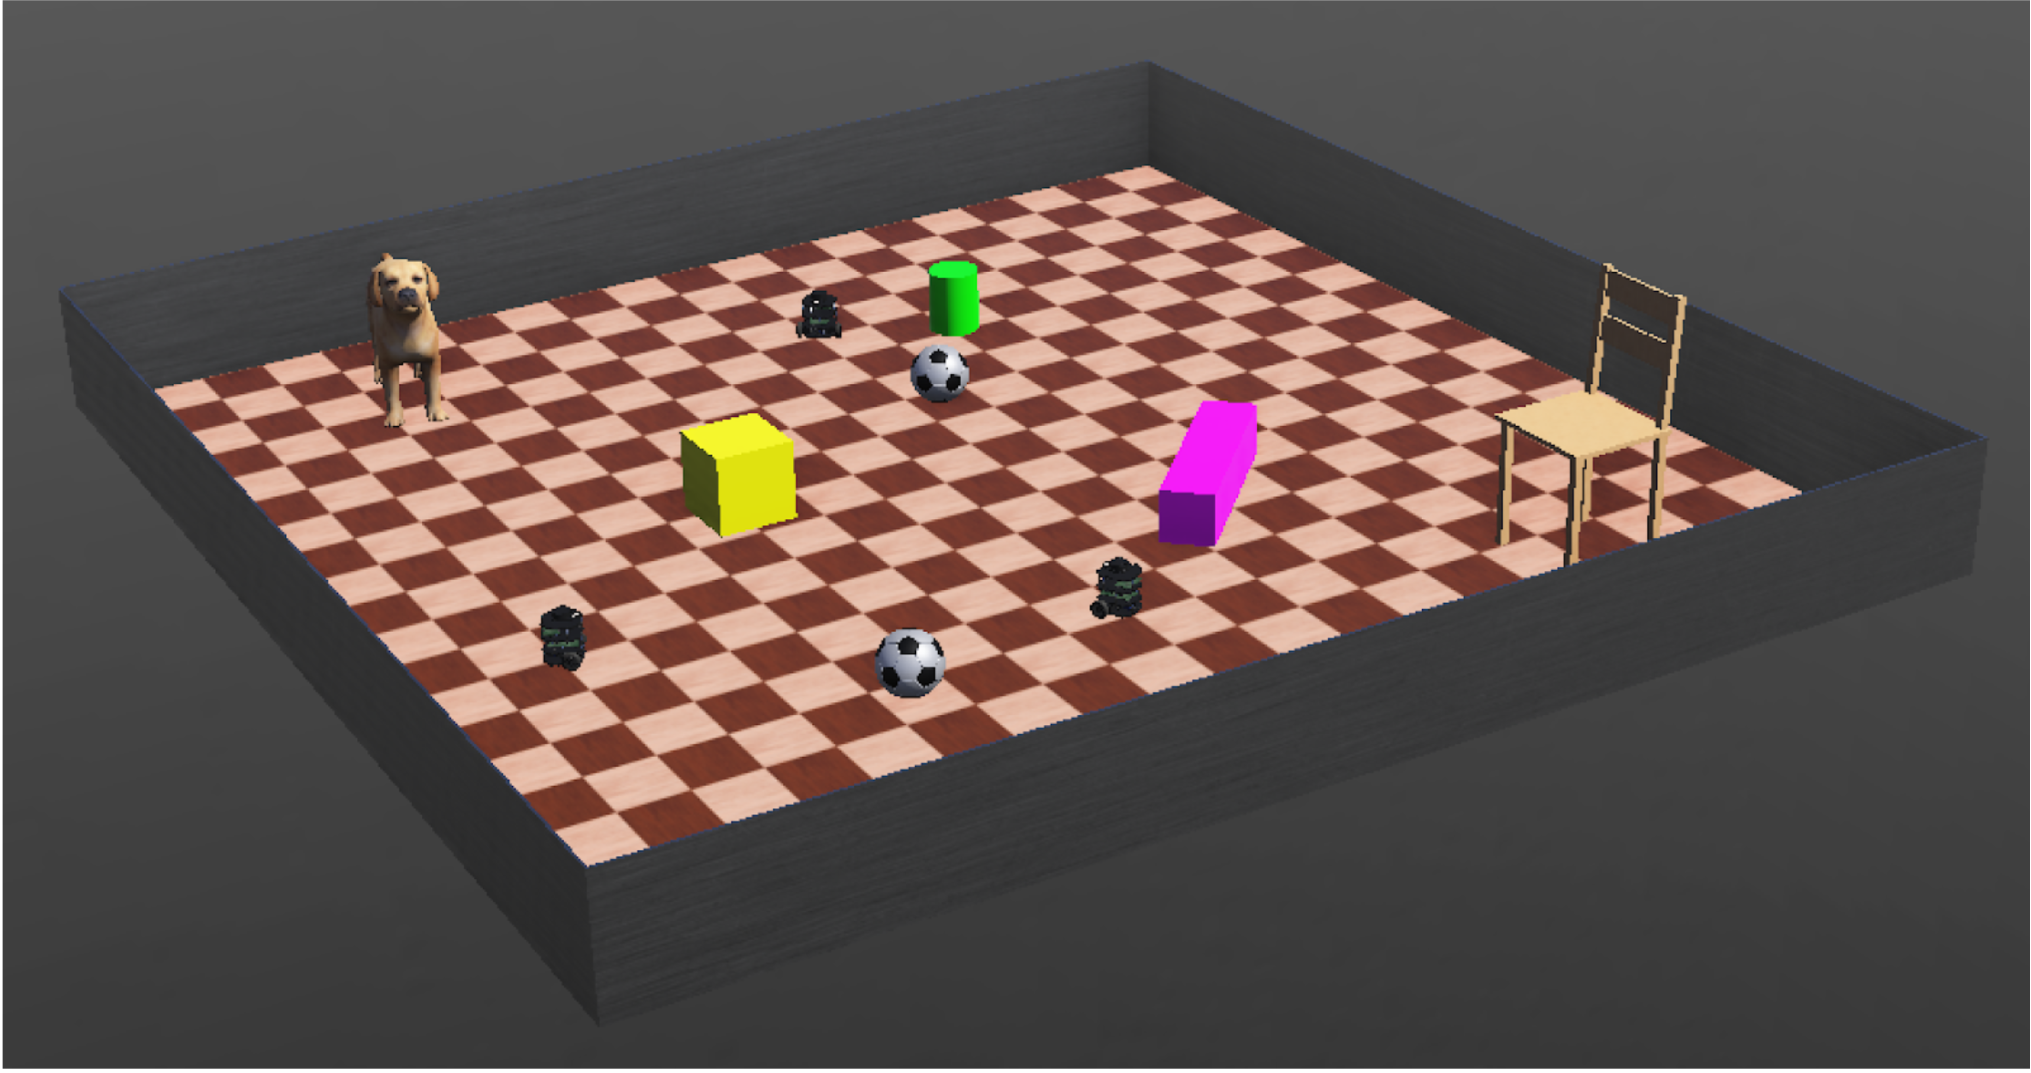
\includegraphics[width=0.9\linewidth]{assets/images/object_detection/Figure2.png}
    \caption{Webots Arena with distinct targets, objects, and three TurtleBots}
    \label{fig:object detection figure 2.} 
\end{figure}

\paragraph*{}
In the first simulation, the Webots environment is a 5x5 meter arena containing three target objects: a pink rectangular prism, a green cylinder, and a yellow cube. Additionally, household items such as a chair and a dog are included to add complexity to the environment. Three TurtleBots , as shown in Figure 1, equipped with RGB cameras and rangefinders (simulating RGB-D cameras) are used to carry out the detection tasks, as shown in Figure 2.

\paragraph*{}
Each robot was placed randomly within the environment and set to move in a simple circular pattern. As the robots navigated the space, they used their sensors to detect their surroundings, displaying images and highlighting detected targets with a bounding box. Detection was performed using the built-in recognition node in the Webots camera, which was configured to identify objects containing the color yellow. The only yellow object in this simulation was a cube. Upon detecting the yellow cube, each robot located its center and aligned it with the center of its camera frame before coming to a stop. The final position for each robot was facing the yellow cube, with the cube centered in the camera’s frame as shown in Figure 3.

\begin{figure}[H]
    \centering
    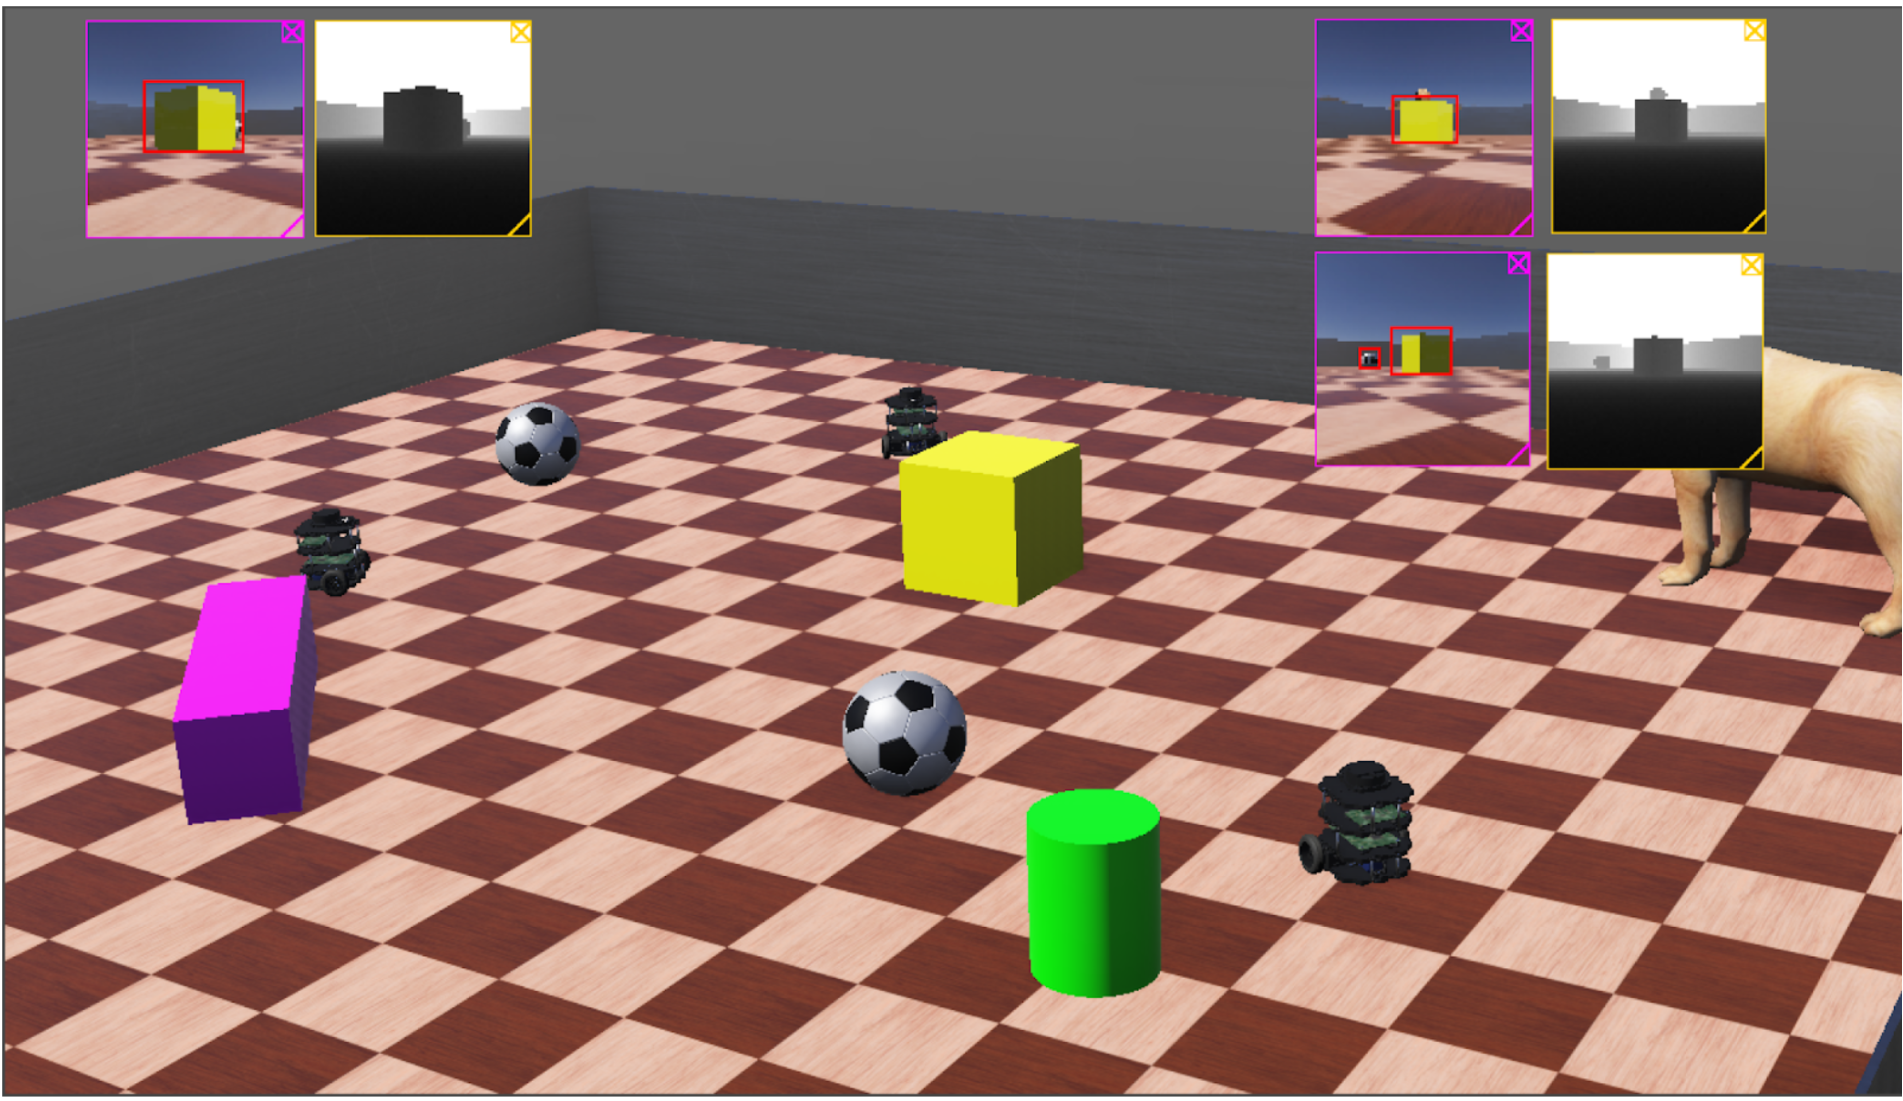
\includegraphics[width=0.8\linewidth]{assets/images/object_detection/Figure3.png}
    \caption{The bounded box is created around detected targets objects (the cube and other 2 geometric shapes) and align the detected yellow cube in the middle of the frame
}
    \label{fig:object detection figure 3.} 
\end{figure}

\paragraph*{}
Additionally, this simulation helped us identify other potential challenges, such as object occlusion, which can interfere with detection. Understanding these challenges early allows us to plan more effective robot pathing and movement strategies in future stages. While object occlusion was not addressed in this phase, it will be considered once color-based object detection is fully operational.

\paragraph*{}
Another key challenge we discovered relates to the physics of balancing the robot when the RGB-D camera is attached. In the simulation, we simplified the setup by using the camera and rangefinder as fixed points attached to the robot to focus solely on object detection and avoid issues with balance. This insight will be addressed in the next phase, where we will implement hardware and ensure proper robot balancing.

\paragraph*{}
Since Webots does not provide any information about the algorithm or model behind its object recognition node, we decided to test a more controllable approach using OpenCV, which was implemented separately in the second simulation.

\section{The Second Simulation}
\textit{Focusing Solely on Color Detection}

\paragraph*{}
In this simulation, the arena only contains one target which is a yellow cube and a TurtleBot the RGB-D camera and the rangefinder attached on it as shown in Figure 4.

\begin{figure}[H]
    \centering
    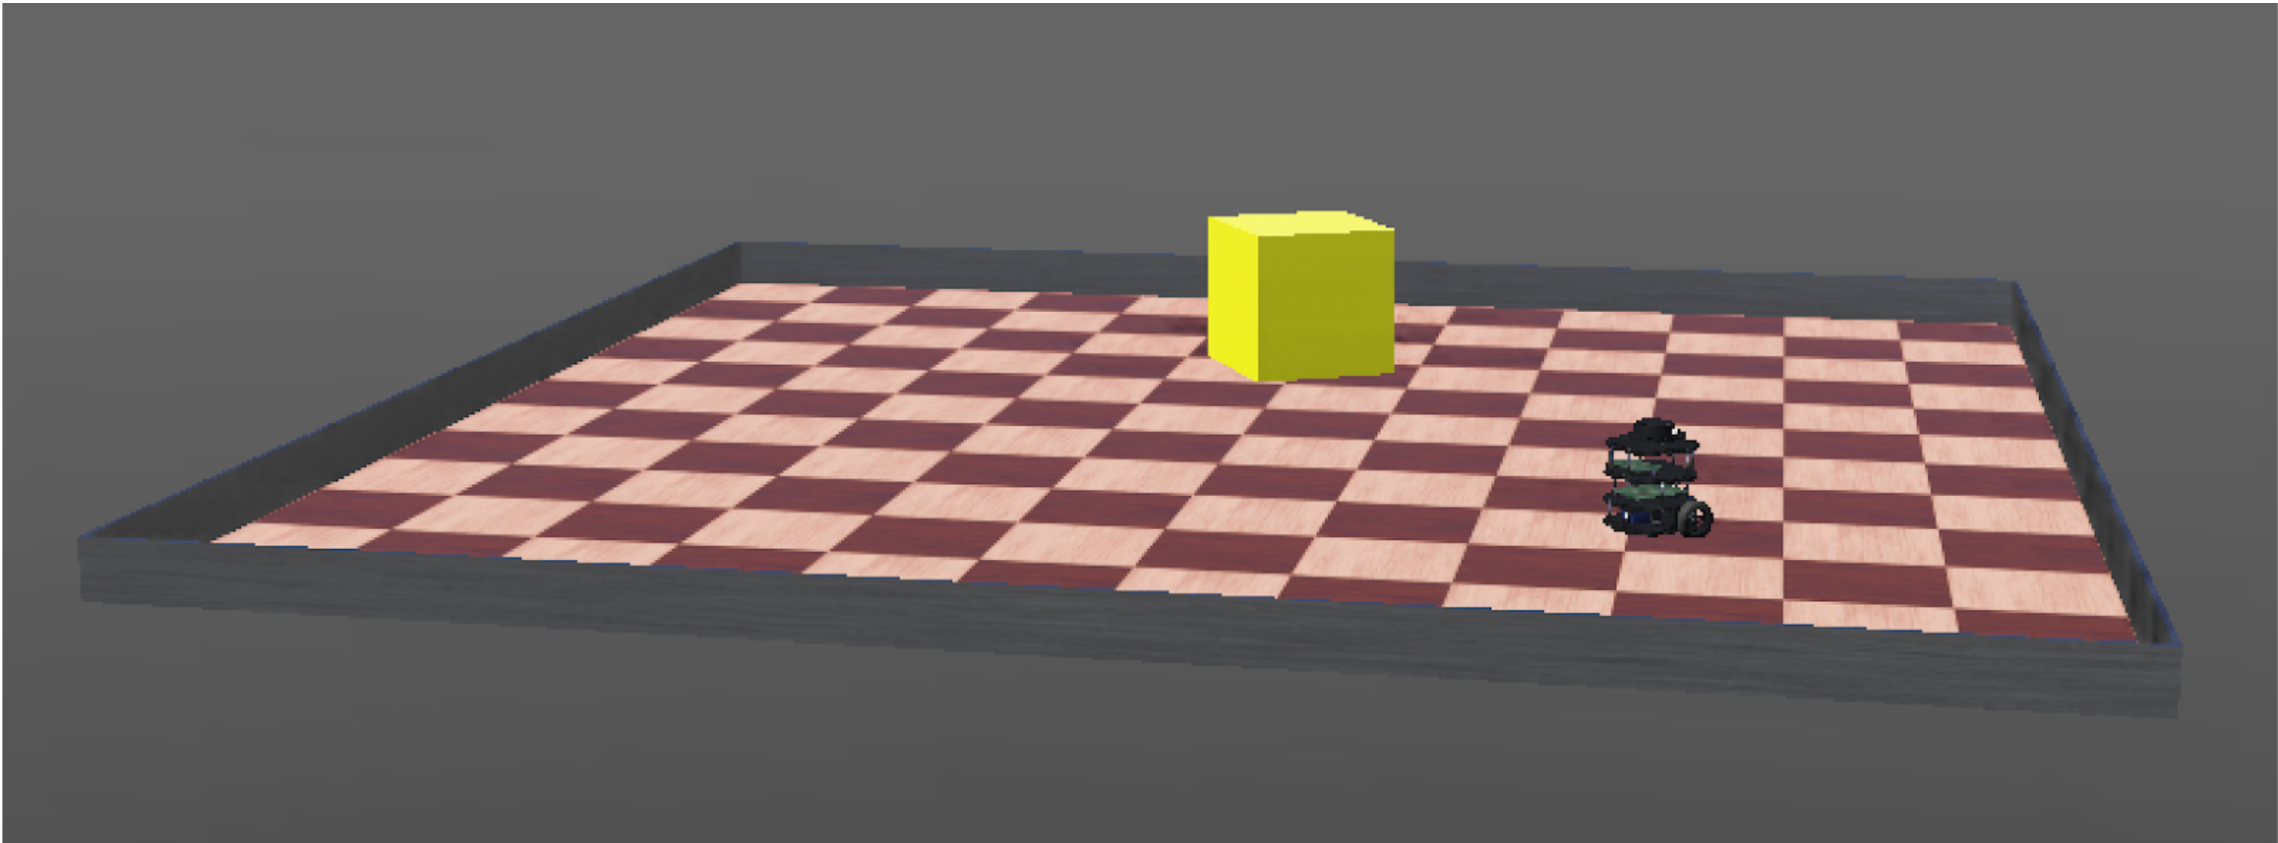
\includegraphics[width=0.8\linewidth]{assets/images/object_detection/Figure4.png}
    \caption{The arena of our second simulation}
    \label{fig:object detection figure 4.} 
\end{figure}

\paragraph*{}
We utilized the HSV model, which is part of OpenCV, to detect objects with the color yellow and draw a bounding box around them. However, one of the key challenges preventing this simulation from working perfectly is the discrepancy between the color code used for the robot and the actual appearance of yellow in the real world. For instance, the yellow RGB code in the real world is (255, 255, 0), but when we applied this same RGB code in the simulation, the resulting color appeared different due to lighting conditions in the virtual environment.

\paragraph*{}
Upon closer observation, we noticed a color shift, meaning the conversion of RGB to HSV in the simulation was not accurate. As a result, only parts of the object fell within the manually set range to match the yellow RGB code used for the box in the simulation. This issue led to partial detection, as illustrated in Figure 5.

\begin{figure}[H]
    \centering
    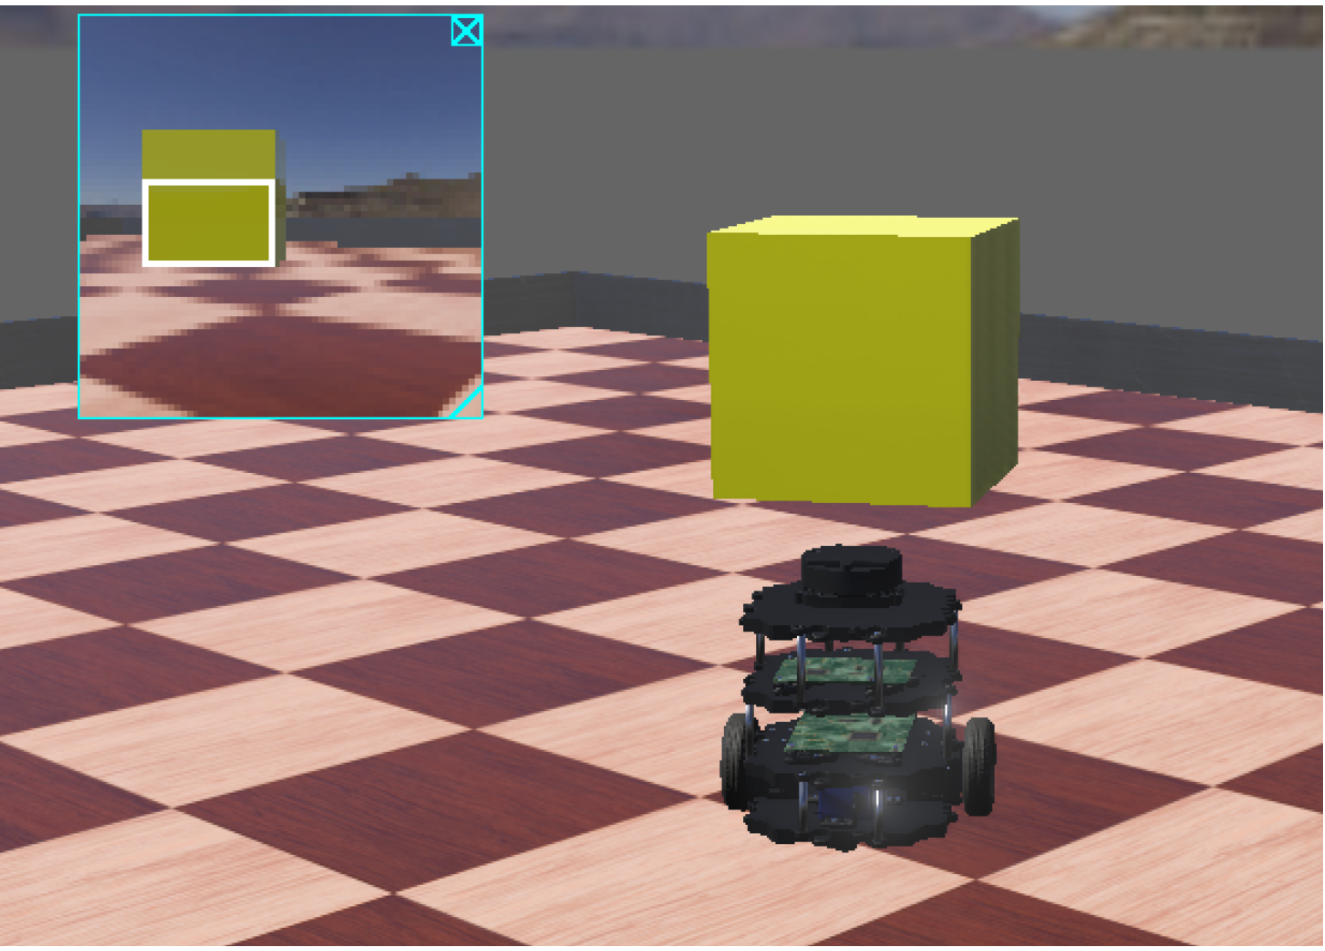
\includegraphics[width=0.8\linewidth]{assets/images/object_detection/Figure5.png}
    \caption{The bounding box created around the target using HSV in OpenCV}
    \label{fig:object detection figure 5.} 
\end{figure}
